
%(BEGIN_QUESTION)
% Copyright 2010, Tony R. Kuphaldt, released under the Creative Commons Attribution License (v 1.0)
% This means you may do almost anything with this work of mine, so long as you give me proper credit

\noindent
{\bf Programming Challenge and Comparison -- Conveyor start/stop control with safety switch} 

\vskip 10pt

Suppose we wish to control the starting and stopping of a large conveyor belt at a factory using a PLC.  This control system will use a ``Start'' pushbutton, a ``Stop'' pushbutton, and an emergency shut-down pull-cable allowing anyone along the conveyor's length to stop the belt simply by tugging on a steel cable (this is akin to the ``stop'' cable used on public buses for passengers to signal to the driver their intent to get off at the next stop).

\begin{itemize}
\item{} {\bf Inputs} 
\item{} Start pushbutton (momentary NO) -- {\it pushing this button closes the switch to energize the PLC input}
\item{} Stop pushbutton (momentary NC) -- {\it pushing this button opens the switch to de-energize the PLC input}
\item{} Emergency stop cable (latching NC) -- {\it tugging on the cable opens the switch to de-energize the PLC input}
\end{itemize}

\begin{itemize}
\item{} {\bf Outputs} 
\item{} Motor contactor -- {\it energizing this PLC output starts the conveyor belt motor}
\end{itemize}

Write a PLC program performing this function, and demonstrate its operation using switches connected to its inputs to simulate the discrete inputs in a real application.  

\vskip 10pt

When your program is complete and tested, capture a screen-shot of it as it appears on your computer, and prepare to present your program solution to the class in a review session for everyone to see and critique.  The purpose of this review session is to see multiple solutions to one problem, explore different programming techniques, and gain experience interpreting PLC programs others have written.  When presenting your program (either individually or as a team), prepare to discuss the following points:

\begin{itemize}
\item{} Identify the ``tag names'' or ``nicknames'' used within your program to label I/O and other bits in memory
\item{} Follow the sequence of operation in your program, simulating the system in action
\item{} Identify any special or otherwise non-standard instructions used in your program, and explain why you decided to take that approach
\item{} Show the comments placed in your program, to help explain how and why it works
\item{} How you designed the program (i.e. what steps you took to go from a concept to a working program)
\end{itemize}

\vskip 20pt \vbox{\hrule \hbox{\strut \vrule{} {\bf Suggestions for Socratic discussion} \vrule} \hrule}

\begin{itemize}
\item{} How do you keep the motor ``latched'' on when the momentary ``Start'' switch is released?
\item{} Which is simpler: implementing this function using normal program coils, or implementing this function using retentive coils (``set'' and ``reset'', or ``latch'' and ``unlatch'')?
\end{itemize}

\vfil 

\underbar{file i02340}
\eject
%(END_QUESTION)





%(BEGIN_ANSWER)

Two different program solutions:

$$\includegraphics[width=15.5cm]{i02340x01.eps}$$

%(END_ANSWER)





%(BEGIN_NOTES)



%INDEX% PLC, programming challenge: conveyor start/stop with safety switch

%(END_NOTES)




